% Name: Hilbert curve
% Description: The fifth step of the Hilbert curve, a path through every cell of a 32 by 32 grid that keeps neighbors on the path close in the square.
% Tags: Hilbert curve, space-filling curve, fractal, L-system

\usetikzlibrary{lindenmayersystems}

\pgfdeclarelindenmayersystem{Hilbert curve}{
  \rule{A -> +BF-AFA-FB+}
  \rule{B -> -AF+BFB+FA-}}

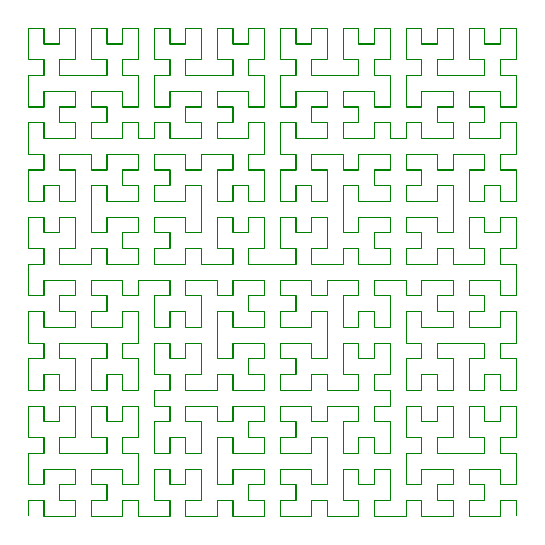
\begin{tikzpicture}
  % Order 5 visits 2⁵ × 2⁵ cells, so the curve spans 31 steps of 2 mm each way
  \draw[green!50!black, line join=round, lindenmayer system={Hilbert curve, axiom=A, order=5, angle=90, step=2mm}] lindenmayer system;
\end{tikzpicture}
